\chapter{Fundamentals}

Before proceeding to examine the automation script more in details, it will be necessary to explain what are the main ingredients of this framework. However most of the game take place in the web site xnat. 
XNAT is an open source imaging informatics platform developed by the Neuroinformatics Research Group at Washington University. It facilitates common management, productivity, and quality assurance tasks for imaging and associated data. Thanks to its extensibility, XNAT can be used to support a wide range of imaging-based projects.\footnote{https://www.xnat.org/about/}, Due to the fact that xnat is offering the opportunity to Use the power of high-performance computing on your data, subsequently  pipeline processing is on of the option that can be done on xnat. As well as the deployment of the docker container.
\\
Additionally XNAT has a structured web site that is composed from a Dashboard that give a overview over the web site, a Project list that browses or search available projects, and a Project page where all subjects and their data in this project are, with  manage members, view project resources. Along with Subject/Session pages where all details for are given , imaging session, scan-level detail.
As well as the part of the scans where all the scans of the patient are found. 
this Structure of XNAT provides the information where the patients file are stored including the composed URL for the REST API use. 
\\
A container is a standard unit of software that packages up code and all its dependencies so the application runs quickly and reliably from one computing environment to another. A Docker container image is a lightweight, standalone, executable package of software that includes everything needed to run an application: code, runtime, system tools, system libraries and settings.\footnote{https://www.docker.com/resources/what-container/}
A docker container allows the user to deploy any applications in any environment without worrying about incompatible issues regardless of the machine’s configuration settings.\footnote{https://sematext.com/glossary/docker/} Although there is some associate terms that will always be needed when it comes to using or learning about Docker container.
One the top of them is the Dockerfile, the dockerfile is a file that contains the build instruction for the image that the Docker Engine( Docker Engine is an open source containerization technology for building and containerizing your applications.\footnote{https://docs.docker.com/engine/}) will run. Conversely there is numerous commands that must be written  the dockerfile in order to create the image. After proceeding with building the image we can Tag and push the image to the docker hub. for the purpose of doing that we just have to run some basic simple commands on a Terminal.\\
Another element to consider is the REST APIS, A REST API is an application programming interface (API) that follows the design principles of the REST architectural style. REST is short for representational state transfer, and is a set of rules and guidelines about how you should build a web API.\footnote{https://www.redhat.com/en/topics/api/what-is-a-rest-api} Luckily xnat is providing his users with a list of XNAT REST APIS that make the exchange between the user an the web site possible. 

At the same time if we want to xnat to execute my created docker image and run run a command on  JSON Command is needed. The JSON  Command is a collection of properties that describes the docker image, which lied xnat to understand what the command  is about. In other word the JSON command is a sort of configuration for the xnat. it answers the folowing  questions for xnat: What kind of image is it? Does it have a human-friendly name we can use for it? What does the command-line string look like? Does it need files? Where should they go? How do you want to get those out of XNAT? Does it produce any files at the end? Those have to get back into XNAT, so where should they go?\footnote{https://wiki.xnat.org/container-service/json-command-definition} Those are the fundamentals knowledge needed in order to achieve a automation of the process. 




\begin{figure}
    \centering
    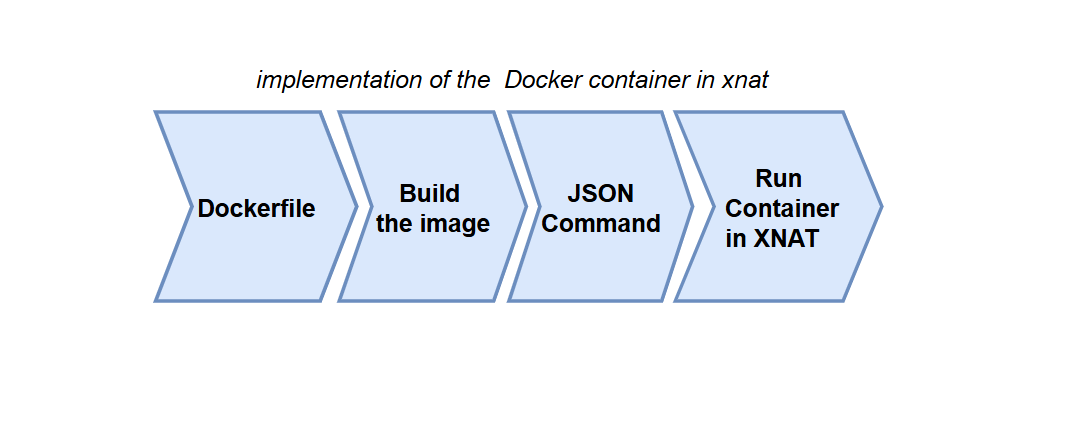
\includegraphics[width=0.9\linewidth]{en/content/ste.png}
    \caption{Diagram: the implementation of the docker Conatiner in xnat}
    \label{fig:enter-label}
\end{figure}





